% sections/05_next_steps.tex: generated by newdeck/html2beamer.py from the HTML deck, then edited by hand

% ---------------------------------------------------------------- slide 34: Outline
\begin{btframe}{}{Outline}
\begin{outlinelist}
\outlineitem{1}{Introduction}{the background types, the geometry, the input muons and neutrinos}{0.35}
\outlineitem{2}{Simulation}{transport, inelastic scattering, technologies, hits and digitisation, signal generation}{0.35}
\outlineitem{3}{Selection}{track cuts, pair cuts and time coincidence}{0.35}
\outlineitem{4}{Backgrounds before tagging}{μ and ν inelastic scattering, MS7 K\textsubscript{L}, combinatorial pairs}{0.35}
\outlineitem{5}{Background tagging}{rules, V0 rule, SBT model, R1, R2, summary}{0.35}
\outlineitem{6}{Optimisation and conclusion}{genetic-algorithm search, the optimised designs Z2 and Z3}{1.00}
\end{outlinelist}
\end{btframe}

% ---------------------------------------------------------------- slide 35: design optimisation with a genetic algorithm (19 Nov 2026)
\begin{btframe}{6 · Optimisation · method}{Design optimisation: a genetic algorithm on the full chain}
\begin{minipage}[t]{0.56\linewidth}\vspace{0pt}
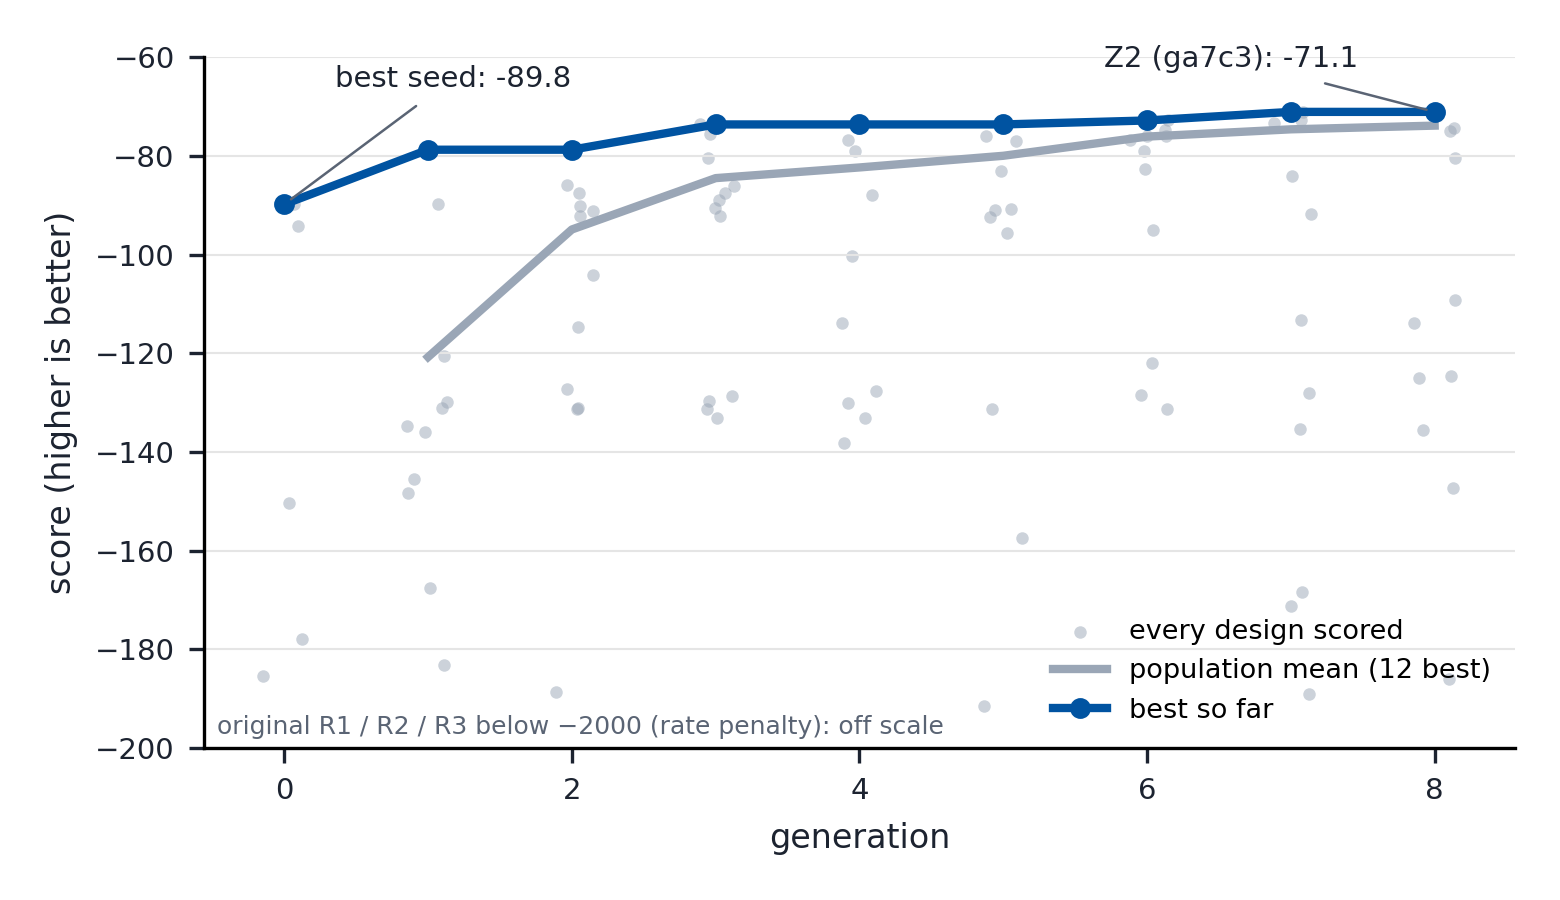
\includegraphics[width=\linewidth]{figs/s35_ga_convergence.png}
\end{minipage}\hfill
\begin{minipage}[t]{0.41\linewidth}\vspace{2pt}
{\fontsize{6.15pt}{8.60pt}\selectfont
\begin{itemize}
  \item \textbf{Genes}: SBT rings and threshold, UBT straw extent, tile plane size and 2×2 / 4×4 cm regions, V0 rule settings
  \item \textbf{Each generation}: 12 children by crossover + mutation, scored on Slurm with the chain of this talk (10\textsuperscript{5} signal decays); keep the 12 best
  \item \textbf{Score}: background left, signal lost, cost, rate limits; and the untagged fraction of bounced single SST1 muons
  \item \textbf{Seeds}: the reference designs and R1 / R2 with a 3.4 m tile plane, 2×2 cm only in the cavern-side flame block
  \item Model fixed; V0 p\textsubscript{max} cut held on
\end{itemize}}
\end{minipage}
\slidenote{Source: veto evolve/ga\_designs.py, lib/veto/objective.py (code 56a0e20); run results\_rerun/evolve/ga\_20261119\_115533 (8 × 12, 1 h on the UZH farm). Best 5 re-scored with 2 more signal seeds: Z2 (ga7c3) −71.0 ± 0.5.}
\end{btframe}

% ---------------------------------------------------------------- slide 31: Z2: R2 without the SBT, 7 straw fins per side — 439.7 drachmas, 193 368 channels
\begin{btframe}{6 · Optimisation · Z2}{Z2 (optimised): SBT 6 rings + UBT + V0 rule — 225.3 drachmas, 21 171 channels}
{\centering {\renewcommand{\skubtlabel}{UBT: straws + tiles |x| < 1.7 m, 2 × 2 cm\textsuperscript{2} only on the cavern side}\designsketch[74.52pt]{2,5,6,7,8,9}{0}{SBT: rings 2, 5–9 (6 of 10)}}\par}
\vspace{2.46pt}
\noindent \begin{minipage}[c]{0.5\linewidth}
{\fontsize{5.31pt}{6.90pt}\selectfont\setlength{\tabcolsep}{3.72pt}\renewcommand{\arraystretch}{1.42}
\begin{tabular}{lr}
\textcolor{muted}{per 15 y, full selection} & \textcolor{muted}{Z2} \\\headrule
signal lost, full IP cut & 2.71 \% \\\rowrule
combinatorial pairs & 0 simulated pairs left \\\rowrule
μ in the vessel & 1.3 ± 1.3 (1 event) \\\rowrule
ν in the helium & 1.13 ± 0.11 \\\rowrule
SBT material & 0.004 ± 0.003 \\\rowrule
\rowcolor{tint}\bfseries MS7 (μ V0, K\textsuperscript{±}, ν) & \bfseries 0.80 ± 0.34 \\\rowrule
single SST1 muons tagged, all / bounced & 91 / 84 \% \\\rowrule
\end{tabular}\par}
\end{minipage}%
\hfill%
\begin{minipage}[c]{0.5\linewidth}
{\fontsize{6.15pt}{8.60pt}\selectfont
\begin{itemize}
  \item Best design of the genetic-algorithm search (section 6): R2 with 6 of the 10 SBT rings (no 0, 1, 3, 4)
  \item UBT straws with t\textsubscript{0} and the segment cut; tile plane |x| < 1.7 m, 2×2 cm only on the cavern side
  \item V0 rule with a 15.7 mrad cone, no K\textsubscript{L} time-of-flight window, p\textsubscript{max} kept
  \item \textbf{Signal loss 2.7 \%} (R2: 6.7 \%), 68 \% of the budget; every plane within its rate limit
\end{itemize}}
\end{minipage}\par
\end{btframe}

% ---------------------------------------------------------------- slide 32: Z3 (optimised)
\begin{btframe}{6 · Optimisation · Z3}{Z3 (optimised): SBT 7 rings + UBT + V0 rule — 244.7 drachmas, 22 428 channels}
{\centering {\renewcommand{\skubtlabel}{UBT: straws + tiles |x| < 1.7 m, 2 × 2 cm\textsuperscript{2} only on the cavern side}\designsketch[74.52pt]{2,3,5,6,7,8,9}{0}{SBT: rings 2, 3, 5–9 (7 of 10)}}\par}
\vspace{2.46pt}
\noindent \begin{minipage}[c]{0.5\linewidth}
{\fontsize{5.31pt}{6.90pt}\selectfont\setlength{\tabcolsep}{3.72pt}\renewcommand{\arraystretch}{1.42}
\begin{tabular}{lr}
\textcolor{muted}{per 15 y, full selection} & \textcolor{muted}{Z3} \\\headrule
signal lost, full IP cut & 3.01 \% \\\rowrule
combinatorial pairs & 0 simulated pairs left \\\rowrule
μ in the vessel & 1.3 ± 1.3 (1 event) \\\rowrule
ν in the helium & 1.05 ± 0.10 \\\rowrule
SBT material & 0.004 ± 0.003 \\\rowrule
\rowcolor{tint}\bfseries MS7 (μ V0, K\textsuperscript{±}, ν) & \bfseries 0.61 ± 0.27 \\\rowrule
single SST1 muons tagged, all / bounced & 94 / 84 \% \\\rowrule
\end{tabular}\par}
\end{minipage}%
\hfill%
\begin{minipage}[c]{0.5\linewidth}
{\fontsize{6.15pt}{8.60pt}\selectfont
\begin{itemize}
  \item Second design of the search: as Z2 with ring 3 back (7 rings)
  \item MS7 0.61 and single SST1 tagging 94 \% (Z2: 0.80, 91 \%) for +19 drachmas
  \item \textbf{Signal loss 3.0 \%}, 73 \% of the budget
\end{itemize}}
\end{minipage}\par
\slidenote{Optimised design (ga8c8 of run results\_rerun/evolve/ga\_20261119\_115533, re-scored −75.9 ± 5.9 over 3 seeds); design file results\_rerun/evolve/Z3\_opt\_ga8c8.json. Evaluated with the optimiser chain (full selection, UBT rate ×1).}
\end{btframe}

% ---------------------------------------------------------------- slide 35b: optimisation result
\begin{btframe}{6 · Optimisation · result}{Optimised designs Z2 and Z3: same tagging, half the signal loss, 68–73 \% of the budget}
{\fontsize{5.31pt}{6.90pt}\selectfont\setlength{\tabcolsep}{3.72pt}\renewcommand{\arraystretch}{1.42}
\begin{tabularx}{\linewidth}{>{\raggedright\arraybackslash}Xrrr}
\textcolor{muted}{per 15 y, full selection} & \textcolor{muted}{R2, 3.4 m tiles (seed)} & \textcolor{muted}{\textbf{Z2} (ga7c3)} & \textcolor{muted}{Z3 (ga8c8)} \\\headrule
cost, drachmas (\% of budget) & 303.8 (91 \%) & \textbf{225.3 (68 \%)} & 244.7 (73 \%) \\\rowrule
SBT rings & all 10 & 2, 5–9 & 2, 3, 5–9 \\\rowrule
V0 cone / time-of-flight window & 25 mrad / on & 15.7 mrad / off & 15.7 mrad / off \\\rowrule
μ in the vessel & 1.3 (1 ev.) & 1.3 (1 ev.) & 1.3 (1 ev.) \\\rowrule
SBT material & 2.95 ± 2.99 (1 heavy ev.) & 0.004 & 0.004 \\\rowrule
MS7 μ (V0, K\textsuperscript{±}) & 0.59 ± 0.25 & 0.80 ± 0.34 & 0.61 ± 0.27 \\\rowrule
ν in the helium & 1.08 & 1.13 & 1.05 \\\rowrule
single SST1 tagged, all / bounced & 94 / 83 \% & 91 / 84 \% & 94 / 84 \% \\\rowrule
\rowcolor{tint}\bfseries signal lost & \bfseries 5.94 \% & \bfseries 2.71 \% & \bfseries 3.01 \% \\\rowrule
\end{tabularx}\par}
\vspace{2.46pt}
{\fontsize{6.15pt}{8.60pt}\selectfont
\begin{itemize}
  \item Solid: signal loss halved (5.9 → 2.7 \%) and −79 drachmas, with the bounced-muon tagging kept; every plane within its rate limit
  \item The SBT-material gain is one heavy simulated event: not a measured improvement
  \item All three keep the same changes: rings 0, 1, 4 off, straw t\textsubscript{0} + segment cut, tighter V0 cone
\end{itemize}}
\slidenote{Source: results\_rerun/evolve/ga\_20261119\_115533/history.jsonl, confirm.json; objective with bounced-SST1 weight 100. Tiles |x| < 1.7 m: cavern-side 2×2 cm block 0.30 MHz / channel (limit 2.5), +x 4×4 cm block 0.92 MHz (limit 1). Reference designs unchanged.}
\end{btframe}

% ---------------------------------------------------------------- slide 36: Conclusion
\begin{btframe}{6 · Next steps · conclusion}{Conclusion}
{\fontsize{6.15pt}{8.60pt}\selectfont
\begin{itemize}
  \item Full chain on the Nov-4 production: muon and neutrino inelastic scattering, MS7 K\textsubscript{L}, combinatorial pairs with muons, rock and interaction products
  \item Before tagging the MS7 K\textsubscript{L} dominate (1.8×10\textsuperscript{4} / 15 y), then the vessel muon interactions (2×10\textsuperscript{3}) and the rock × μ pairs (211)
  \item \textbf{R2} (SBT + UBT + V0 rule, at the budget) removes everything that enters through a wall and, with the V0 rule, the MS7 and SBT-material K\textsubscript{L}: \textasciitilde{}3 events left, mostly neutrinos, at 6.7 / 9.7 \% signal loss
  \item \textbf{One muon event in the helium} left in R2 (1.3 / 15 y): a 157 GeV muon kinked by 5 mrad at z = 73.8 m; its straight backward line misses its own UBT hit by 20 cm (window 7 cm). No vertex cone in the designs: it would cost signal
  \item The signal loss is set by random hits: the UBT and SBT rates are the key systematic
  \item \textbf{Optimisation} (genetic algorithm, full chain): Z2 keeps R2's tagging at 68 \% of the budget and halves the signal loss (2.7 \%)
  \item Next: enriched samples for the one-event classes (vessel μ, SBT material); FairShip validation of the optimum
\end{itemize}}
\end{btframe}
